\documentclass{article}
\usepackage[utf8]{inputenc}
\usepackage{amsmath}
\usepackage{amsfonts}
\usepackage{xeCJK}

\title{自主浮空器的容错控制研究}
\author{肖畅}
\date{2017年6月24日}

\begin{document}

\maketitle

\section{问题概述及研究价值}
\subsection{飞行器容错控制研究的必要性}
飞行器的发明至今已有100多年的历史。人类已经发展出了适应于不同飞行高度和任务的多种飞行器。在20km高度以下,通常以固定翼飞机、直升飞机和中低空飞艇为主;在高度100km以上,通常以卫星为主;而在20km-100km的高度通常以平流层飞艇、浮空器为主。飞行器按照功能又可分为载人飞行器和无人飞行器:载人飞行器在民航运输、太空探测领域的应用前景宽广;而无人飞行器在抢险救灾、卫星通信等领域有巨大的潜力。在军事方面,飞行器还可用于敌情侦查,危险区域探测、执行无人任务、充当通信中继平台等方面。

但是,自从飞行器发明以来,系统故障就是一个不可避免的话题。由于系统长时间运行、材料设备老化、系统过于复杂甚至飞行员操作失误等多种原因,任何飞行器都会在运行过程中发生故障。尤其是飞行器被大量用于民航领域之后,空难代价十分巨大。因此提高飞行器的自主性、减少人为干预、并提出有效的容错控制方案,是十分必要的。

事实上,由于设计、制造飞行器耗费资金巨大,其安全运行一直被工程师和科学家们重视。在上世纪90年代以前,人们已经熟知通过设计冗余的执行机构,进行对多输入多输出(MIMO)的系统的反馈控制器设计\cite{makarand1988actuator,conner1979fail}。但是控制器的表现都不太理想。甚至是明知在控制器故障之后,剩余控制器有足够能力保持系统稳定的前提下,控制系统仍然无法让被控对象保持稳定\cite{119629}。因此,设计一个能够容忍执行机构或传感器故障,并保持系统闭环行为的控制系统,在20世纪80年代的时候开始成为学术研究的热点。

飞行器的容错控制意义非常深远。无论商用还是军用飞行器,都搭载了十分复杂的控制系统。由于系统的复杂性,许多零部件不可避免地会发生不可预知的错误;而不同系统之间的互相依赖、不同变量之间的耦合都会将任何一个小故障放大,甚至影响飞行安全。因此,针对飞行器的容错控制的研究意义十分重大。

\subsection{容错控制与鲁棒控制的不同}
鲁棒控制(Robust Control)与容错控制最为本质的区别在于,前者主要处理的是系统模型中的参数小扰动或者建模本身忽略了一些因素带来的不确定性;后者主要处理的是一些由于系统故障造成的更加猛烈的变化。鲁棒控制与容错控制再算法上有相似的地方,因此有些鲁棒控制的算法可以稍加修改后,应用到容错控制中来,如Ackermann\cite{ackermann2012sampled,ackermann2012robust}和Siljak\cite{4789828}在参数空间法上的工作。

\section{相关领域研究现状}
飞行器的容错控制是非线性系统容错控制的一个分支,非线性系统的容错在国内外也已经有很多研究成果。飞行器的容错控制研究,没有跳出非线性系统的范畴,研究方法也与非线性系统类似。现在学术界对容错控制的分类方法有一些不同的观点。Blanke等\cite{BLANKE1997693}从工程角度把容错控制系统分成三层——底层(控制层)、中层(探测与重构)和高层(监测)。许域菲\cite{xuyufei2011}对比了增益预置(Gain Scheduling)、特征结构配置(Eigenvector Assignment)、自适应控制(Adaptive control)、滑模变结构控制(Sliding mode control)、反演思想(Backstepping)和智能控制(Intelligence control)这六种先进容错控制方法的优缺点。Yin在做航天器姿态容错控制的工作中,认为将容错控制分为故障检测与控制器重构\cite{7407616}。尽管这些分类方法从不同角度阐述了容错控制的研究现状,但是目前最主流的分类是将容错控制根据设计思路不同分为被动容错控制和主动容错控制\cite{Zhang2008229,5160615,jiang2005fault,gaozhifeng2011,xuyufei2011,wangdejun2014},文献\cite{Jiang201260}阐述了被动容错与主动容错的本质上的不同,本文也采纳这一分类观点。而其中主动容错控制又可分为故障检测与诊断和容错控制器设计两个步骤,目前这两个步骤也各自都是相关领域的研究热点。在具体的控制器设计方法上,被动容错控制和主动容错控制有很多相似之处。本文中,\ref{subsec:passive}主要介绍非线性系统的被动容错研究;\ref{subsec:fdd}介绍故障检测与诊断的研究成果;\ref{subsec:active}主要介绍非线性系统的主动控制研究成果;\ref{subsec:aircraftftc}主要介绍\ref{subsec:passive}和\ref{subsec:active}未涉及到的飞行器控制研究。

\subsection{被动容错控制}\label{subsec:passive}
\subsubsection{被动容错控制的概念}
被动容错控制(Passive Fault-tolerant Control, PFTC),其思想是针对一种或几种错误,使用鲁棒控制的一些技巧,构造一个控制器,使得这几种已知错误发生时对控制器的影响减到最小或忽略不计\cite{jiang2005fault,6859271}。在PFTC中,“被动”表示控制器一旦构造好就不再改变事先设计好的参数和结构,当系统发生任何被考虑在内的故障时,这个控制器能自动对故障进行补偿,保证系统的闭环动态品质在一个可接受的范围内。其优点是运算速度快、无需掌握错误的在线信息,一切运算都在离线时算好,控制器实施起来较为简单;缺点是必须事先想好错误发生的种类和影响,并将其表现在系统模型的参数变化中,只能应对已知的几种错误,无法应对不可预知类型的错误。同时,由于被动容错需要用一种控制器应对多种错误,那么这种控制器势必要设计得非常保守,因而很难达到最优控制效果\cite{jiang2005fault}。

为了直观地说明被动容错控制的思想,在此引用文献\cite{Jiang201260}中的一张示意图——图\ref{fig:asp}表示了不同错误下的一个控制器空间示意图。其中三个大圆表示三种错误下,能够保持系统的可接受的控制器范围。每种错误都有一个对应的最优控制器解(图中Optimal solution)。我们如果要设计一种被动容错控制器,同时处理这三种错误,那么只能将控制器设计在图中三圆的公共区域(图中阴影区域)。显然,这对三种错误来说各自都不是最优解,可以说需要处理的错误种类越多,系统的相应距离最优解越遥远。特别是图\ref{fig:aspoverlap}所示的几种情况,三个圆没有交集,那么理论上针对这样系统的被动容错控制是不存在的,这时只能对错误进行取舍。
\begin{figure}[!htp]
    \centering
    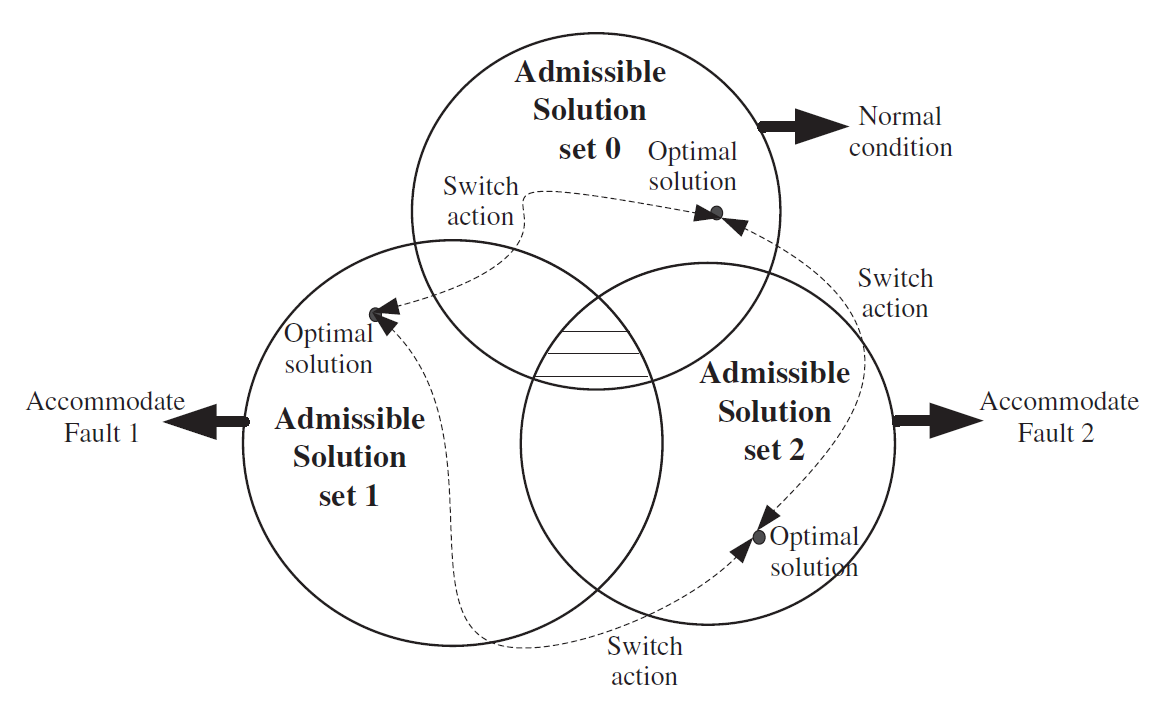
\includegraphics[width = 0.6\textwidth]{admissiblesp.png}
    \caption{可接受的控制空间示意\cite{Jiang201260}}
    \label{fig:asp}
\end{figure}
\begin{figure}[!htp]
    \centering
    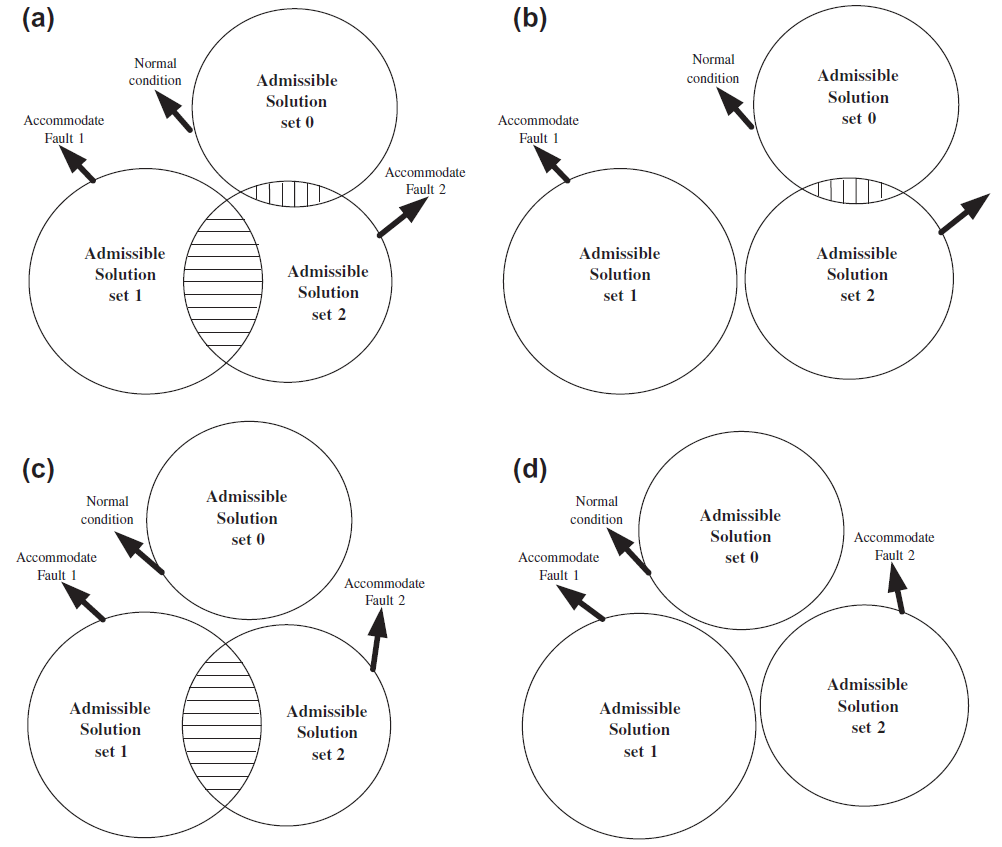
\includegraphics[width = 0.6\textwidth]{aspoverlap.png}
    \caption{其他控制器空间示意\cite{Jiang201260}}
    \label{fig:aspoverlap}
\end{figure}

\subsubsection{被动容错控制的发展}
被动容错控制文献中被称为可靠控制(Reliable control)。“可靠”的概念第一次由Siljak于1980年提出\cite{siljak1980},经过Date和Cho等人的发展\cite{70346,4790503},最终在1992年由Robert J. Veillette进行系统地总结\cite{119629},提出了“可靠控制”这一概念。往后,文献中的凡是以被动容错控制思路设计的控制器,都以reliable control呈现。

被动容错控制的设计方法有很多种,在$H_\infty$优化\cite{119629,7850999}、LMI方法\cite{7795198,974340,1236798}、LQ方法\cite{VEILLETTE1995137,847106,866928},滑模控制方法\cite{4160860},模糊系统\cite{7795198,7505963,Zha20173267},动态预补偿结合特征结构配置\cite{Jiang2000Design,ZHAO19981267},去中心化观测器\cite{70346}等方面均有相关研究成果。其中文献\cite{ZHAO19981267}首次给控制器冗余和错误构建了数学模型。另外,根据针对系统错误的不同,被动容错控制还可以分为针对执行机构失效\cite{ZHAO19981267,974340,VEILLETTE1995137,1236798,Tian20101907,Li20132455,7353144,7863042,70346,866928}、时变错误\cite{7850999,CHEN2004349,6064886}和随机错误\cite{7795198,7505963,5540530,Zha20173267}。

国内外也有不少文献对被动容错控制提出了分类方法。国外文献中,Fekih\cite{6859271}用鲁棒控制的分类方法把被动容错控制分为了数量反馈理论法、$H_\infty$范数优化法\cite{4079591}、LQ控制法\cite{Staroswiecki20072070}、$\mu$同步法和变结构方法。国内文献中,王德军\cite{wangdejun2014}、许德智\cite{xudezhi2013}和高志峰\cite{gaozhifeng2011}都将被动容错控制分为可靠镇定、完整性与联立镇定三类方法。肖冰\cite{xiaobing2014}认为在航天器姿态控制中,被动容错控制可以与主动容错控制的控制器重构部分做为一个方向共同研究。他将航天器姿态容错控制方法,分为基于自适应技术(Adaptive)的方法、基于滑模控制的方法和基于控制分配的方法三类,这一点在Yin. S的论文中\cite{7407616}也得到了有力的支撑。

\subsection{故障检测与诊断}\label{subsec:fdd}
故障检测(Fault Detection)与故障诊断(Fault Diagnosis)是两个不同的概念。故障检测,一般指系统对是否发生故障进行在线检测;而故障诊断,指的是在检测到故障的基础上,判断故障的类型和严重性。故障检测与诊断是主动容错控制器设计前的必经步骤。其中故障检测现在最为常用的方法,是设计一个残差(Residual)函数。通过残差函数的输出值,结合统计学来判断系统出了哪一类故障。因此,残差函数的设计就显得尤为重要,是故障检测的核心步骤。而残差函数的设计方法,通常可以分为两大类——基于模型的方法和基于数据的方法。故障诊断则更偏向于一种分类方法。
\subsection{主动容错控制}\label{subsec:active}
主动容错控制的思想是通过在线辨识系统控制设备的状态,估计控制器的错误类型,并针对已发生的错误种类,实时生成能够让系统继续保持稳定的控制器。主动容错控制系统一般分为两个步骤:故障检测以及控制器生成。故障检测又可分为两大类——基于模型和不基于模型的;控制器生成可以分为三大类——控制器池法,控制分配方法

\subsubsection{基于控制分配的容错控制}
通常,一个有冗余的控制器可以建模如\eqref{eq:adundantnonmodel}
\begin{equation}\label{eq:adundantnonmodel}
\tau = h(u,x,t)
\end{equation}
其中$h$是控制器函数,$\tau \in \mathbb{R}^m$,$u\in \mathbb{U} \subset \mathbb{R}^p$ 是控制输入,而$\mathbb{U}$代表控制器的取值空间,$\mathbb{R}^p$代表$p$维线性空间。控制分配方法的主要思想是通过安置冗余的控制器或传感器,在一个或多个设备出现故障的时候(即$u$无法达到期望取值的时候),及时调整控制器的输入$u$,使得控制器的输出$\tau$维持不变或变动很小。鉴于控制器设计的时候留有冗余,因此通常情况下有$p>m$。
\subsubsection{第二类主动容错}
\subsubsection{第三类主动容错}
\subsubsection{第四类主动容错}
\subsection{飞行器容错}\label{subsec:aircraftftc}



\section{研究方法}
\subsection{拟解决的关键问题}
\subsection{现有的研究手段}
\subsection{问题的难点}

\section{论文目录}

\bibliographystyle{unsrt}
\bibliography{MyBib_Control}

\end{document}
